\documentclass[aspectratio=169, 10pt]{beamer}

% ---------- Theme ----------
\usetheme{metropolis}
\usepackage{appendixnumberbeamer}

% ---------- Packages ----------
\usepackage[utf8]{inputenc}
\usepackage[T1]{fontenc}
\usepackage{graphicx}
\usepackage{booktabs}
\usepackage{amsmath,amssymb}
\usepackage{tikz}
\usetikzlibrary{arrows.meta, positioning, calc}
\usepackage{xcolor}
\usepackage{colortbl}

% ---------- Colors ----------
\definecolor{accent}{HTML}{2E86AB}
\definecolor{danger}{HTML}{D7263D}
\definecolor{success}{HTML}{2A9D8F}
\definecolor{warn}{HTML}{E9C46A}
\setbeamercolor{frametitle}{bg=accent!95!black, fg=white}
\setbeamercolor{progress bar}{fg=accent}
\setbeamercolor{alerted text}{fg=danger}

% ---------- Metadata ----------
\title{Hash-Based Digital Signatures}
\subtitle{Lamport OTS \(\to\) WOTS \(\to\) Merkle Signature Scheme}
\author{Aicha Slaitane \and Abdullah Algethami}
\institute{Applied Cryptography (CS 232) --- KAUST}
\date{}

\begin{document}

% ====================================================================
% TITLE
% ====================================================================
\maketitle

% ====================================================================
% OUTLINE
% ====================================================================
\begin{frame}{Outline}
\begin{columns}[t]
\begin{column}{0.48\textwidth}
\begin{enumerate}
    \item Motivation: The Quantum Threat
    \item Lamport One-Time Signatures
    \item Winternitz OTS (WOTS)
    \item Merkle Signature Scheme
    \item Hypertrees
\end{enumerate}
\end{column}
\begin{column}{0.48\textwidth}
\begin{enumerate}\setcounter{enumi}{4}
    \item OTS Benchmarks
    \item Key-Reuse Attack
    \item MSS Performance Evaluation
    \item Parameter Tuning
    \item Hypertrees
    \item Conclusion
\end{enumerate}
\end{column}
\end{columns}
\end{frame}

% ====================================================================
% PART 1 --- AICHA
% ====================================================================
\section{Theory \& Implementation}

% ---- Slide: Motivation ----
\begin{frame}{The Quantum Threat}
\begin{columns}
\begin{column}{0.55\textwidth}
\begin{itemize}
    \item \textbf{Shor's algorithm} (1994) breaks RSA, ECDSA, and Diffie--Hellman in polynomial time on a quantum computer.
    \item These schemes rely on the hardness of \emph{factoring} or \emph{discrete logs}.
    \item \alert{We need signatures based on different assumptions.}
\end{itemize}
\vspace{6pt}
\textbf{Hash-based signatures} rely \emph{only} on the one-wayness of hash functions (e.g.\ SHA-256).
\begin{itemize}
    \item No number-theoretic assumptions.
    \item Grover's algorithm gives only a \(\sqrt{}\) speedup \(\Rightarrow\) SHA-256 still provides \(\sim\)128-bit quantum security.
\end{itemize}
\end{column}
\begin{column}{0.42\textwidth}
\centering
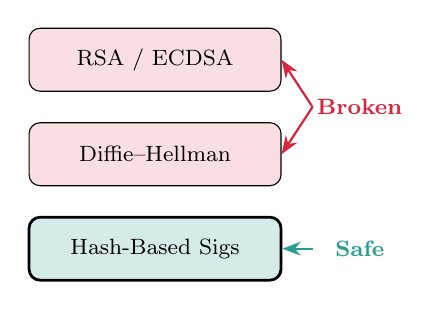
\begin{tikzpicture}[
    box/.style={draw, rounded corners, minimum width=3.2cm, minimum height=0.8cm, align=center, font=\footnotesize},
    >=Stealth
]
\node[box, fill=danger!15] (rsa) at (0,2.4) {RSA / ECDSA};
\node[box, fill=danger!15] (dh) at (0,1.2) {Diffie--Hellman};
\node[box, fill=success!20, line width=1pt] (hbs) at (0,0) {Hash-Based Sigs};
\node[font=\footnotesize\bfseries, text=danger] at (2.6,1.8) {Broken};
\node[font=\footnotesize\bfseries, text=success] at (2.6,0) {Safe};
\draw[->, thick, danger] (2.0,1.8) -- (rsa.east);
\draw[->, thick, danger] (2.0,1.8) -- (dh.east);
\draw[->, thick, success] (2.0,0) -- (hbs.east);
\end{tikzpicture}
\end{column}
\end{columns}
\end{frame}

% ---- Slide: Lamport Overview ----
\begin{frame}{Lamport One-Time Signature}
\textbf{Key Generation:} \textit{(Where $H$ is a cryptographic collision resistant hash function e.g. SHA-256)}
\begin{columns}
\begin{column}{0.52\textwidth}
\vspace{4pt}

\begin{itemize}
    \item Generate 256 pairs of random 32-byte blocks.
    \item Secret key: \(\text{SK}[i] = (s_i^0,\; s_i^1)\)
    \item Public key: \(\text{PK}[i] = \bigl(H(s_i^0),\; H(s_i^1)\bigr)\)
\end{itemize}
\vspace{6pt}
\textbf{Signing} message \(m\):
\begin{enumerate}
    \item Compute \(h = H(m)\) --- 256 bits.
    \item For each bit \(h_i\), reveal \(s_i^{h_i}\).
\end{enumerate}
\vspace{6pt}
\textbf{Verification:}\\
Check \(H(\sigma_i) \stackrel{?}{=} \text{PK}[i][h_i]\) for all \(i\).
\end{column}
\begin{column}{0.45\textwidth}
\centering
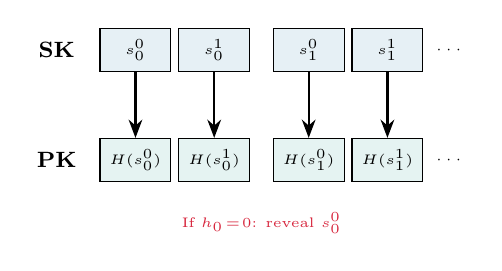
\begin{tikzpicture}[
    sk/.style={draw, fill=accent!12, minimum width=0.9cm, minimum height=0.55cm, font=\tiny},
    pk/.style={draw, fill=success!12, minimum width=0.9cm, minimum height=0.55cm, font=\tiny},
    >=Stealth
]
% Labels
\node[font=\footnotesize\bfseries] at (-0.4,2.6) {SK};
\node[font=\footnotesize\bfseries] at (-0.4,1.2) {PK};
% SK row
\node[sk] (s00) at (0.6,2.6) {$\scriptscriptstyle s_0^0$};
\node[sk] (s01) at (1.6,2.6) {$\scriptscriptstyle s_0^1$};
\node[sk] (s10) at (2.8,2.6) {$\scriptscriptstyle s_1^0$};
\node[sk] (s11) at (3.8,2.6) {$\scriptscriptstyle s_1^1$};
\node[font=\tiny] at (4.6,2.6) {$\cdots$};
% PK row
\node[pk] (p00) at (0.6,1.2) {$\scriptscriptstyle H(s_0^0)$};
\node[pk] (p01) at (1.6,1.2) {$\scriptscriptstyle H(s_0^1)$};
\node[pk] (p10) at (2.8,1.2) {$\scriptscriptstyle H(s_1^0)$};
\node[pk] (p11) at (3.8,1.2) {$\scriptscriptstyle H(s_1^1)$};
\node[font=\tiny] at (4.6,1.2) {$\cdots$};
% Arrows
\draw[->, thick] (s00) -- (p00);
\draw[->, thick] (s01) -- (p01);
\draw[->, thick] (s10) -- (p10);
\draw[->, thick] (s11) -- (p11);
% Highlight
\node[font=\tiny, text=danger] at (2.2,0.4) {If $h_0\!=\!0$: reveal $s_0^0$};
\end{tikzpicture}
\end{column}
\end{columns}

\vspace{6pt}
\begin{block}{Key Properties}
Signature = 8,192\,B \quad|\quad Signing: 0.03\,ms (no hashing!) \quad|\quad \alert{Strictly one-time use}
\end{block}
\end{frame}

% ---- Slide: Lamport Limitation ----
\begin{frame}{Why Is Lamport One-Time?}
\begin{itemize}
    \item Each signature reveals \textbf{256 of 512} secret blocks.
    \item A second signature on a different message reveals \emph{different} blocks.
    \item After \(k\) reuses, an attacker has collected enough blocks to forge \emph{any} message.
\end{itemize}

\vspace{8pt}
\begin{center}
\begin{tabular}{ccc}
\toprule
\textbf{Reuses ($k$)} & \textbf{Blocks Exposed} & \textbf{Forgery Probability} \\
\midrule
1 & 50\% & $\approx 0\%$ \\
8 & 99.6\% & 38.5\% \\
10 & 99.9\% & 78\% \\
15 & 100\% & $>$99.9\% \\
\bottomrule
\end{tabular}
\end{center}

\vspace{4pt}
\centering
\textbf{Two solutions:} \quad (1) Use WOTS to reduce sizes \quad (2) Use Merkle trees to manage many keys
\end{frame}

% ---- Slide: WOTS 1 ----
\begin{frame}{Winternitz OTS: The Hash Chain}
\vspace{2pt}
\textbf{Recall the problem with Lamport:} it signs the message \emph{one bit at a time}, so the signature is large (8\,KB).

\vspace{4pt}
\textbf{Winternitz idea:} sign \emph{several bits at once} as a small number (a ``digit''), using a \emph{hash chain}.

\vspace{8pt}
\textbf{A hash chain} is one secret value hashed over and over. Each arrow applies $H$ once:

\vspace{10pt}
\centering
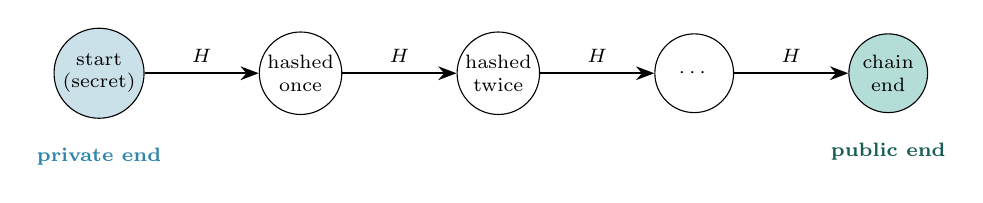
\begin{tikzpicture}[
    node distance=1.45cm,
    val/.style={draw, circle, minimum size=1.0cm, inner sep=1pt, font=\scriptsize, align=center},
    >=Stealth
]
\node[val, fill=accent!25] (sk) {start\\(secret)};
\node[val, right=of sk] (h1) {hashed\\once};
\node[val, right=of h1] (h2) {hashed\\twice};
\node[val, right=of h2] (hd) {$\cdots$};
\node[val, right=of hd, fill=success!35] (pk) {chain\\end};

\draw[->, thick] (sk) -- (h1) node[midway, above, font=\scriptsize] {$H$};
\draw[->, thick] (h1) -- (h2) node[midway, above, font=\scriptsize] {$H$};
\draw[->, thick] (h2) -- (hd) node[midway, above, font=\scriptsize] {$H$};
\draw[->, thick] (hd) -- (pk) node[midway, above, font=\scriptsize] {$H$};

\node[below=0.25cm of sk, font=\scriptsize\bfseries, text=accent] {private end};
\node[below=0.25cm of pk, font=\scriptsize\bfseries, text=success!60!black] {public end};
\end{tikzpicture}

\vspace{8pt}
\footnotesize
Moving \textbf{forward} is easy (just hash). Moving \textbf{backward} is infeasible (it would mean inverting $H$). This one-way direction is what makes the chain secure.
\end{frame}

% ---- Slide: WOTS 2 ----
\begin{frame}{WOTS: Signing One Digit (Toy Example, $w=4$)}
\vspace{2pt}
One chain signs \textbf{one digit} $d \in \{0,1,2,3\}$. The position along the chain \emph{is} the digit value.

\vspace{4pt}
\begin{itemize}
    \item \textbf{Private value:} the start of the chain (random, kept secret).
    \item \textbf{Public value:} the end of the chain --- the start hashed $w\!-\!1 = 3$ times.
    \item \textbf{To sign digit $d$:} reveal the value at position $d$ (the start hashed $d$ times).
    \item \textbf{To verify:} hash the revealed value the remaining $3-d$ times --- it must reach the public value.
\end{itemize}

\vspace{6pt}
\centering
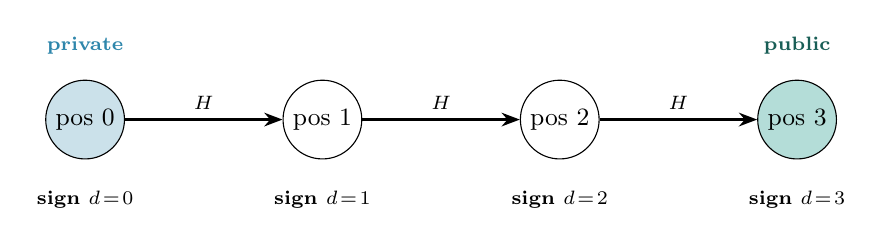
\begin{tikzpicture}[
    node distance=2.0cm,
    hash/.style={draw, circle, minimum size=1.0cm, inner sep=0, font=\small},
    >=Stealth
]
\node[hash, fill=accent!25] (sk) {pos 0};
\node[hash, right=of sk] (h1) {pos 1};
\node[hash, right=of h1] (h2) {pos 2};
\node[hash, right=of h2, fill=success!35] (pk) {pos 3};

\draw[->, thick] (sk) -- (h1) node[midway,above,font=\scriptsize]{$H$};
\draw[->, thick] (h1) -- (h2) node[midway,above,font=\scriptsize]{$H$};
\draw[->, thick] (h2) -- (pk) node[midway,above,font=\scriptsize]{$H$};

\node[above=0.2cm of sk, font=\scriptsize\bfseries, text=accent] {private};
\node[above=0.2cm of pk, font=\scriptsize\bfseries, text=success!60!black] {public};

\node[below=0.28cm of sk, font=\scriptsize\bfseries] {sign $d\!=\!0$};
\node[below=0.28cm of h1, font=\scriptsize\bfseries] {sign $d\!=\!1$};
\node[below=0.28cm of h2, font=\scriptsize\bfseries] {sign $d\!=\!2$};
\node[below=0.28cm of pk, font=\scriptsize\bfseries] {sign $d\!=\!3$};
\end{tikzpicture}

\vspace{6pt}
\footnotesize
\alert{But one chain only signs one digit.} A real message hash has many digits --- so WOTS uses \textbf{many chains in parallel} (next slide).
\end{frame}

% ---- Slide: WOTS 2b --- THE FULL KEY ----
\begin{frame}{WOTS: The Full Key is Many Chains}
\vspace{2pt}
The message hash is split into many digits --- and \textbf{each digit gets its own chain}. With $w\!=\!16$, that is 67 chains side by side.

\vspace{6pt}
\centering
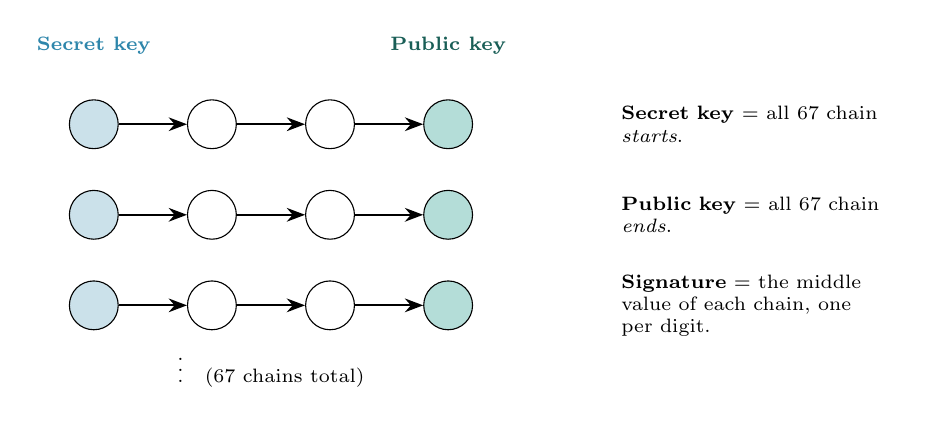
\begin{tikzpicture}[
    node distance=1.2cm and 1.5cm,
    sv/.style={draw, circle, minimum size=0.62cm, inner sep=0, font=\tiny, fill=accent!25},
    mid/.style={draw, circle, minimum size=0.62cm, inner sep=0, font=\tiny},
    pv/.style={draw, circle, minimum size=0.62cm, inner sep=0, font=\tiny, fill=success!35},
    >=Stealth
]
% three example chains
\foreach \r/\y in {1/0, 2/-1.15, 3/-2.3} {
  \node[sv]  (s\r) at (0, \y)   {};
  \node[mid] (a\r) at (1.5, \y) {};
  \node[mid] (b\r) at (3.0, \y) {};
  \node[pv]  (p\r) at (4.5, \y) {};
  \draw[->, thick] (s\r) -- (a\r);
  \draw[->, thick] (a\r) -- (b\r);
  \draw[->, thick] (b\r) -- (p\r);
}
\node[font=\scriptsize] at (2.25, -3.05) {$\vdots$ \; (67 chains total)};
% braces / labels
\node[font=\scriptsize\bfseries, text=accent, align=center] at (0, 1.0) {Secret key};
\node[font=\scriptsize\bfseries, text=success!60!black, align=center] at (4.5, 1.0) {Public key};
\node[font=\scriptsize, align=left, text width=3.4cm] at (8.4, 0)
  {\textbf{Secret key} = all 67 chain \emph{starts}.};
\node[font=\scriptsize, align=left, text width=3.4cm] at (8.4, -1.15)
  {\textbf{Public key} = all 67 chain \emph{ends}.};
\node[font=\scriptsize, align=left, text width=3.4cm] at (8.4, -2.3)
  {\textbf{Signature} = the middle value of each chain, one per digit.};
\end{tikzpicture}

\vspace{4pt}
\begin{block}{In one sentence}
\small To sign a message: split its hash into digits, and from each chain reveal the value at that digit's position. The verifier finishes every chain and checks all 67 ends match the public key.
\end{block}
\end{frame}

% ---- Slide: WOTS 3 ----
\begin{frame}{WOTS: Why We Need a Checksum}
\vspace{2pt}
\textbf{The problem:} hashing \emph{forward} is free for everyone --- including the attacker.
\begin{itemize}
    \item A signature reveals a value somewhere along each chain.
    \item The attacker can hash it forward and produce a valid value for any \emph{higher} digit.
    \item So, unprotected, an attacker could forge any message whose digits are all $\geq$ ours.
\end{itemize}

\vspace{6pt}
\textbf{The fix: a checksum.} We append a checksum $C = \sum_i (w - 1 - d_i)$ and sign it with extra chains.
\begin{itemize}
    \item Raising any message digit makes the checksum \emph{decrease}.
    \item A smaller checksum digit means going \emph{backward} in a chain --- which needs inverting $H$.
    \item So the attacker is blocked: they cannot raise a digit without breaking the checksum.
\end{itemize}

\vspace{4pt}
\begin{center}
\footnotesize
\begin{tabular}{ccc}
\toprule
$w$ & Chains (incl. checksum) & Signature Size \\
\midrule
4 & 133 & 4,256 B \\
\rowcolor{accent!10}
\textbf{16} & \textbf{67} & \textbf{2,144 B} \\
256 & 34 & 1,088 B \\
\bottomrule
\end{tabular}\\[3pt]
\scriptsize Larger $w$ $\Rightarrow$ fewer chains $\Rightarrow$ smaller signature (but longer chains to compute).
\end{center}
\end{frame}

% ---- Slide: WOTS 4 ----
\begin{frame}{WOTS: The Full Picture}
\vspace{2pt}
Signing a message is just this pipeline --- hash it, split into digits, walk each chain:

\vspace{8pt}
\centering
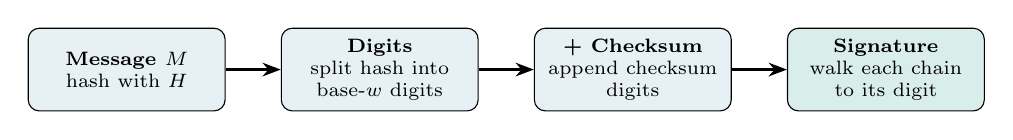
\begin{tikzpicture}[
    node distance=0.7cm,
    stepbox/.style={draw, rounded corners, minimum width=2.5cm, minimum height=1.05cm,
                    align=center, font=\scriptsize, fill=accent!12},
    >=Stealth
]
\node[stepbox] (m) {\textbf{Message $M$}\\hash with $H$};
\node[stepbox, right=of m] (d) {\textbf{Digits}\\split hash into\\base-$w$ digits};
\node[stepbox, right=of d] (cs) {\textbf{+ Checksum}\\append checksum\\digits};
\node[stepbox, right=of cs, fill=success!18] (sg) {\textbf{Signature}\\walk each chain\\to its digit};

\draw[->, thick] (m)  -- (d);
\draw[->, thick] (d)  -- (cs);
\draw[->, thick] (cs) -- (sg);
\end{tikzpicture}

\vspace{10pt}
\begin{columns}[t]
\begin{column}{0.5\textwidth}
\begin{block}{The three keys, defined}
\footnotesize
\textbf{Secret key} --- one random start value per chain.\\[2pt]
\textbf{Public key} --- each start hashed $w\!-\!1$ times (every chain end).\\[2pt]
\textbf{Signature} --- each chain stopped at its digit's position.
\end{block}
\end{column}
\begin{column}{0.5\textwidth}
\begin{block}{Verification}
\footnotesize
Finish every chain from the signature value; all chain ends must equal the public key.
\end{block}
\textbf{\footnotesize Trade-off:} one-time only, but signatures are $4\times$ smaller than Lamport.
\end{column}
\end{columns}
\end{frame}

% ---- Slide: OTS in Merkle Trees ----
\begin{frame}{From OTS/WOTS to the Merkle Signature Scheme}
\textbf{Both Lamport and WOTS are one-time} --- a fresh keypair is needed for every message.

\vspace{6pt}
\textbf{Merkle's fix:} pre-generate $2^h$ OTS keypairs and bind them under a single public key using a hash tree.

\begin{columns}
\begin{column}{0.6\textwidth}
\begin{itemize}
    \item Each OTS public key $\text{PK}_i$ is hashed to form \textbf{leaf} $L_i$ of the tree.
    \item Internal nodes are computed as $H(\text{left} \| \text{right})$.
    \item The \textbf{tree root} is the single MSS public key (32\,B).
    \item To sign message $i$: run OTS$_i$ and attach the auth path ($h$ sibling nodes) to let anyone recompute the root.
\end{itemize}
\vspace{4pt}

\begin{block}{Advantage of WOTS over Lamport}
WOTS ($w\!=\!16$) signatures are $\approx$4$\times$ smaller (2\,144\,B vs.\ 8\,192\,B), directly shrinking the on-wire MSS signature.
\end{block}

\end{column}
\begin{column}{0.46\textwidth}
\centering
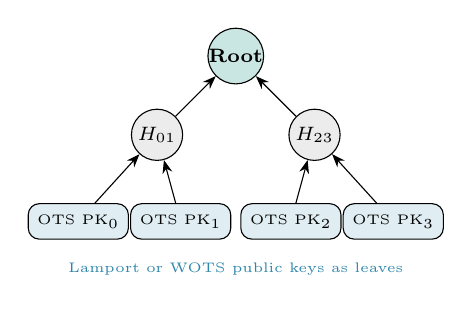
\begin{tikzpicture}[
    nd/.style={draw, circle, minimum size=0.65cm, inner sep=0, font=\scriptsize},
    lf/.style={draw, rectangle, rounded corners, minimum width=1.15cm, minimum height=0.45cm, font=\tiny, align=center},
    >=Stealth]
\node[nd, fill=success!25, font=\scriptsize\bfseries] (root) at (2,3.2) {Root};
\node[nd, fill=gray!15] (h01) at (1,2.2) {$H_{01}$};
\node[nd, fill=gray!15] (h23) at (3,2.2) {$H_{23}$};
\node[lf, fill=accent!15] (l0) at (0,1.1) {OTS PK$_0$};
\node[lf, fill=accent!15] (l1) at (1.3,1.1) {OTS PK$_1$};
\node[lf, fill=accent!15] (l2) at (2.7,1.1) {OTS PK$_2$};
\node[lf, fill=accent!15] (l3) at (4.0,1.1) {OTS PK$_3$};
\draw[->] (h01) -- (root);
\draw[->] (h23) -- (root);
\draw[->] (l0) -- (h01);
\draw[->] (l1) -- (h01);
\draw[->] (l2) -- (h23);
\draw[->] (l3) -- (h23);
\node[font=\tiny, text=accent] at (2,0.5) {Lamport or WOTS public keys as leaves};
\end{tikzpicture}
\end{column}
\end{columns}
\end{frame}

% ---- Slide: Merkle Tree 1 ----
\begin{frame}{Merkle Signature Scheme: Key Generation}
\vspace{4pt}
\textbf{Problem:} One-Time Signatures (OTS) can only sign a single message securely.

\vspace{6pt}
\textbf{Solution:} Build a binary hash tree (Merkle Tree) over \(2^h\) OTS public keys to sign \(2^h\) messages.

\vspace{12pt}
\textbf{Key Generation Process:}
\begin{enumerate}
    \item Generate \(2^h\) independent OTS keypairs.
    \item Hash each OTS public key to form the leaves: \(\text{Leaf}_i = H(\text{OTS\_PK}_i)\).
    \item Compute parent nodes by hashing the concatenation of children: Parent \(= H(\text{left} \| \text{right})\).
    \item The \textbf{MSS public key} is the tree root (just 32\,B).
\end{enumerate}
\end{frame}

% ---- Slide: Merkle Tree 2 ----
\begin{frame}{Merkle Signature Scheme: Sign \& Verify}
\begin{columns}
\begin{column}{0.50\textwidth}
\textbf{To sign} the $i$-th message:
\begin{itemize}
    \item Sign the message with OTS key $i$.
    \item Include the \emph{auth path}: the $h$ sibling hashes needed to reach the root.
\end{itemize}

\vspace{12pt}
\textbf{To verify:}
\begin{itemize}
    \item Verify the underlying OTS signature against $\text{OTS\_PK}_i$.
    \item Reconstruct the root from $\text{Leaf}_i$ and the auth path.
    \item Check if reconstructed root $\stackrel{?}{=}$ MSS public key.
\end{itemize}
\end{column}

\begin{column}{0.48\textwidth}

\centering
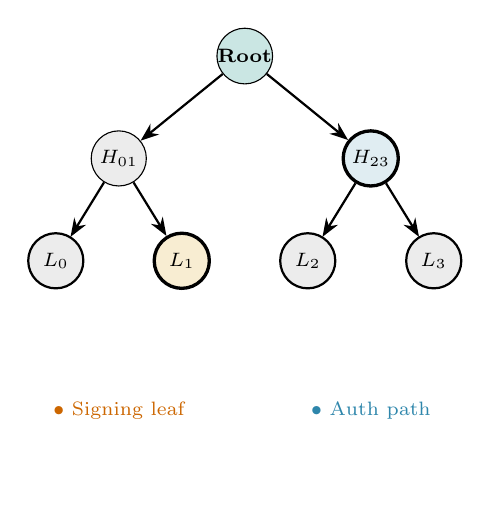
\begin{tikzpicture}[
    level distance=1.3cm,
    sibling distance=1.6cm,
    every node/.style={draw, circle, minimum size=0.7cm, inner sep=0, font=\scriptsize},
    edge from parent/.style={draw, ->, thick},
    level 1/.style={sibling distance=3.2cm},
    level 2/.style={sibling distance=1.6cm},
    >=Stealth
]
\node[fill=success!25, font=\scriptsize\bfseries] {Root}
    child { node[fill=gray!15] {$H_{01}$}
        child { node[fill=gray!15] {$L_0$} }
        child { node[fill=warn!30, line width=1.2pt] {$L_1$} }
    }
    child { node[fill=accent!15, line width=1.2pt] {$H_{23}$}
        child { node[fill=gray!15] {$L_2$} }
        child { node[fill=gray!15] {$L_3$} }
    };

% Legend
\node[draw=none, font=\scriptsize, text=orange!80!black] at (-1.6, -4.5) {$\bullet$ Signing leaf};
\node[draw=none, font=\scriptsize, text=accent] at (1.6, -4.5) {$\bullet$ Auth path};
\end{tikzpicture}

\vspace{6pt}
\footnotesize
Signing leaf $L_1$:\\
Auth path = $[L_0,\; H_{23}]$\\
Verify: $H(H(L_0 \| L_1) \| H_{23}) = \text{Root}$
\end{column}
\end{columns}
\end{frame}

% ---- Slide: Hypertrees (Part 1 introduction) ----
\begin{frame}{Multi-Layer Merkle Trees (Hypertrees)}
\textbf{Problem:} Flat MSS KeyGen builds all $2^h$ OTS keys upfront --- exponentially expensive for large $h$.

\vspace{6pt}
\textbf{Idea:} Stack two Merkle trees. The \emph{top tree} is built immediately; each of its leaves certifies the root of a \emph{bottom tree} that is built \alert{lazily} only when needed.

\begin{columns}
\begin{column}{0.52\textwidth}
\begin{itemize}
    \item Total capacity: $N = 2^{h_{\text{top}} + h_{\text{bot}}}$ messages.
    \item Initial KeyGen: $O(2^{h_{\text{top}}} + 2^{h_{\text{bot}}})$ OTS keys.
    \item Signing produces \emph{two} MSS signatures: one from the bottom tree, one from the top tree certifying the bottom root.
    \item This layering is the core idea behind \textbf{SPHINCS+ / SLH-DSA} (NIST post-quantum standard).
\end{itemize}
\end{column}
\begin{column}{0.44\textwidth}
\centering
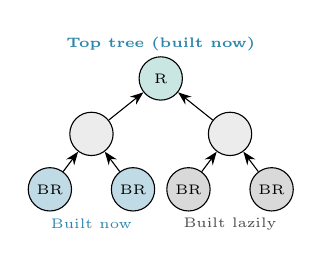
\begin{tikzpicture}[
    nd/.style={draw, circle, minimum size=0.55cm, inner sep=0, font=\tiny},
    >=Stealth, scale=0.88]
\node[font=\tiny\bfseries, text=accent] at (2,4.1) {Top tree (built now)};
\node[nd, fill=success!25] (tr)  at (2,3.6)  {\tiny R};
\node[nd, fill=gray!15]    (tl)  at (1,2.8)  {};
\node[nd, fill=gray!15]    (tr2) at (3,2.8)  {};
\node[nd, fill=accent!30]  (tl1) at (0.4,2.0) {\tiny BR};
\node[nd, fill=accent!30]  (tl2) at (1.6,2.0) {\tiny BR};
\node[nd, fill=gray!30]    (tr1) at (2.4,2.0) {\tiny BR};
\node[nd, fill=gray!30]    (tr3) at (3.6,2.0) {\tiny BR};
\draw[->] (tl)--(tr); \draw[->] (tr2)--(tr);
\draw[->] (tl1)--(tl); \draw[->] (tl2)--(tl);
\draw[->] (tr1)--(tr2); \draw[->] (tr3)--(tr2);
\node[font=\tiny, text=accent] at (1,1.5) {Built now};
\node[font=\tiny, text=gray!60!black] at (3,1.5) {Built lazily};
\end{tikzpicture}
\end{column}
\end{columns}
\end{frame}


% ====================================================================
% PART 2
% ====================================================================
\section{Evaluation \& Extensions}

% ---- Slide: Evaluation Setup ----
\begin{frame}{Evaluation Setup: How Messages Are Generated}
\textbf{Two distinct message generation strategies are used in the evaluation:}

\vspace{8pt}
\begin{columns}

\begin{column}{0.48\textwidth}
\textbf{Security Simulation (Key-Reuse Attack)}
\begin{itemize}
    \item A mix of \textbf{fixed commands} and \textbf{random strings}:
    \begin{itemize}
        \item \small\texttt{"Attack at dawn"}, \texttt{"Hold the line"}\ldots
        \item \small\texttt{f"Random message \{random.random()\}"}
    \end{itemize}
    \item 20 unique messages are signed with the \emph{same} Lamport key.
    \item A fixed target (\texttt{"Retreat at noon"}) tests if a forgery is possible.
    \item Repeated over \textbf{200 independent trials} for statistical validity.
\end{itemize}
\end{column}


\begin{column}{0.48\textwidth}
\textbf{Performance Benchmarking}
\begin{itemize}
    \item A single fixed string is used across all timing trials:
    \begin{block}{}
    \small\texttt{"Post-quantum cryptography is exciting"}
    \end{block}
    \item Each configuration is measured over \textbf{5 repetitions}; we report the \emph{mean and variance} to capture both the typical time and its stability.
    \item The same message is reused across all parameter sweeps for a fair, controlled comparison.
\end{itemize}
\end{column}

\end{columns}
\end{frame}

% ---- Slide: Key-Reuse Attack Theory ----
\begin{frame}{Lamport Key-Reuse Attack}

\begin{columns}


\begin{column}{0.55\textwidth}

\vspace{4pt}

\textbf{Threat model:} A \emph{passive} attacker observes $k$ signatures made with the \textbf{same} Lamport key.

\vspace{6pt}
\begin{itemize}
    \item Each signature reveals one block per position (bit 0 or 1).
    \item After $k$ signatures, the probability a specific block is \emph{still hidden} is $(1/2)^k$.
\end{itemize}

\vspace{6pt}
\textbf{Forgery probability:}
\[
    P_{\text{forge}}(k) = \left(1 - 2^{-k}\right)^{256}
\]

\vspace{4pt}
The attacker needs all 256 blocks matching the target message's hash bits. This converges to certainty exponentially.
\end{column}
\begin{column}{0.42\textwidth}
\centering
\begin{tabular}{ccc}
\toprule
$k$ & $P_{\text{forge}}$ & \textbf{SK Exposed} \\
\midrule
1 & $\approx 0\%$ & 50\% \\
5 & 0.03\% & 96.9\% \\
8 & 38.5\% & 99.6\% \\
10 & 78\% & 99.9\% \\
12 & 94\% & 100\% \\
15 & 99.8\% & 100\% \\
\alert{20} & \alert{100\%} & \alert{100\%} \\
\bottomrule
\end{tabular}

\vspace{6pt}
\footnotesize Results from 200 independent trials per $k$.
\end{column}
\end{columns}
\end{frame}

% ---- Slide: Key-Reuse Empirical Validation ----
\begin{frame}{Empirical Validation}
\begin{columns}
\begin{column}{0.48\textwidth}
\centering
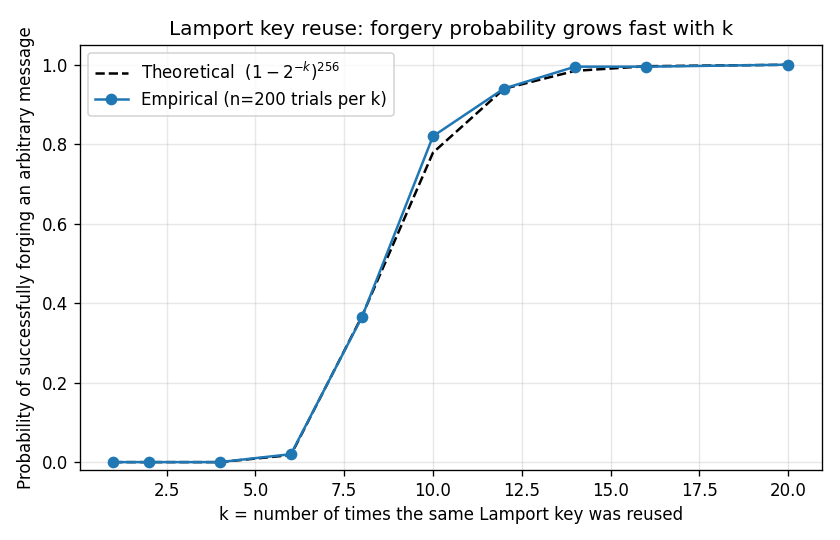
\includegraphics[width=\textwidth]{benchmarks/forgery_probability.png}\\
\footnotesize Empirical vs.\ theoretical forgery rate.\\Theory and experiment match closely.
\end{column}
\begin{column}{0.48\textwidth}
\centering
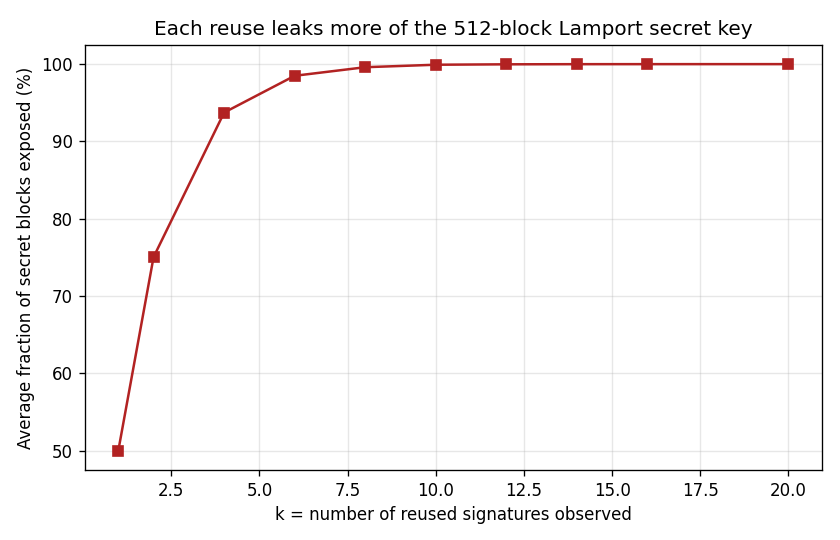
\includegraphics[width=\textwidth]{benchmarks/key_exposure.png}\\
\footnotesize Fraction of SK exposed vs.\ reuse count.\\By $k\!=\!12$ the \alert{complete} key is recovered.
\end{column}
\end{columns}

\vspace{8pt}
\centering
\end{frame}

% ---- Slide: OTS Benchmark Table ----
\begin{frame}{OTS Performance Comparison}
\begin{center}
\footnotesize
\begin{tabular}{lrrrrr}
\toprule
\textbf{Scheme} & \textbf{KG (ms)} & \textbf{Sign (ms)} & \textbf{Verify (ms)} & \textbf{Sig (B)} & \textbf{PK (B)} \\
\midrule
Lamport          & $0.74 \pm 0.013$ & $0.02 \pm 0.000$ & $0.13 \pm 0.002$ & 8,192 & 16,384 \\
WOTS $w\!=\!4$   & $0.29 \pm 0.000$ & $0.11 \pm 0.000$ & $0.10 \pm 0.000$ & 4,256 & 4,256 \\
\rowcolor{accent!10}
WOTS $w\!=\!16$  & $0.40 \pm 0.000$ & $0.19 \pm 0.000$ & $0.18 \pm 0.000$ & 2,144 & 2,144 \\
WOTS $w\!=\!64$  & $1.06 \pm 0.011$ & $0.43 \pm 0.000$ & $0.55 \pm 0.000$ & 1,440 & 1,440 \\
WOTS $w\!=\!256$ & $3.00 \pm 0.006$ & $1.56 \pm 0.021$ & $1.56 \pm 0.014$ & 1,088 & 1,088 \\
\bottomrule
\end{tabular}
\end{center}

\vspace{4pt}
\footnotesize Times reported as \textbf{mean $\pm$ variance} over 5 runs. The very small variances confirm the measurements are stable.

\vspace{4pt}
\normalsize
Key observations:
\begin{itemize}
    \item Lamport signing is extremely fast (0.02\,ms) --- no hash computation, only copying blocks.
    \item WOTS $w\!=\!256$ is \textbf{7.5$\times$ smaller} but much slower than Lamport.
    \item \colorbox{accent!10}{$w\!=\!16$ is the practical sweet spot} --- adopted by XMSS and SPHINCS+.
\end{itemize}
\end{frame}

% ---- Slide: OTS Plots ----
\begin{frame}{OTS: Size vs.\ Speed Trade-off}
\begin{columns}
\begin{column}{0.48\textwidth}
\centering
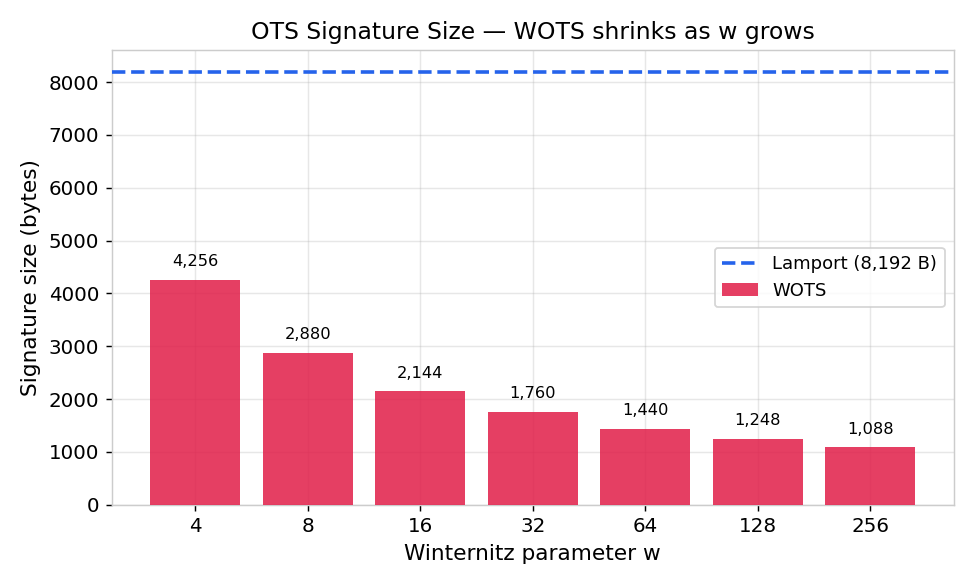
\includegraphics[width=\textwidth]{benchmarks/ots_sig_size.png}\\
\footnotesize Signature size decreases \emph{logarithmically} with $w$.
\end{column}
\begin{column}{0.48\textwidth}
\centering
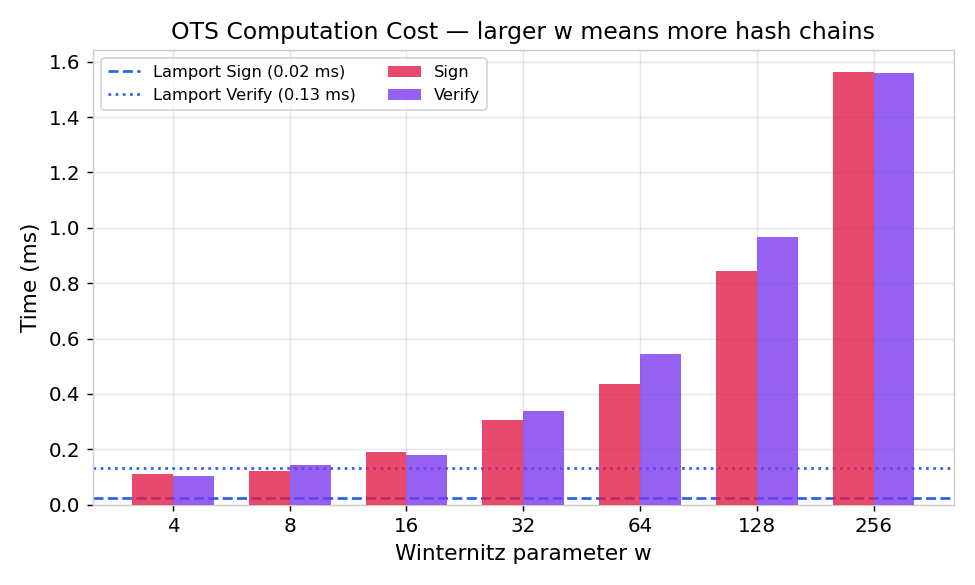
\includegraphics[width=\textwidth]{benchmarks/ots_times.png}\\
\footnotesize Computation time grows \emph{linearly} --- each chain is $w\!-\!1$ hashes long.
\end{column}
\end{columns}
\end{frame}

% ---- Slide: MSS Height Table ----
\begin{frame}{MSS Performance: Scaling with Tree Height}
\begin{center}
\footnotesize
\begin{tabular}{crrrr}
\toprule
\textbf{Height $h$} & \textbf{Messages} & \textbf{KG (ms)} & \textbf{Sign (ms)} & \textbf{Sig Size (B)} \\
\midrule
\multicolumn{5}{c}{\textit{Lamport leaves}} \\
\midrule
4 & 16  & $11.96 \pm 0.01$  & $0.03 \pm 0.00$ & 24,640 \\
6 & 64  & $48.73 \pm 0.71$  & $0.04 \pm 0.00$ & 24,704 \\
8 & 256 & $196.28 \pm 10.19$ & $0.06 \pm 0.00$ & 24,768 \\
\midrule
\multicolumn{5}{c}{\textit{WOTS ($w\!=\!16$) leaves}} \\
\midrule
4 & 16  & $7.11 \pm 0.03$   & $0.21 \pm 0.00$ & 4,420 \\
6 & 64  & $27.99 \pm 0.17$  & $0.22 \pm 0.00$ & 4,484 \\
8 & 256 & $112.17 \pm 1.13$ & $0.23 \pm 0.00$ & 4,548 \\
\bottomrule
\end{tabular}
\end{center}
\vspace{3pt}
\footnotesize Times reported as \textbf{mean $\pm$ variance} over 5 runs.

\vspace{3pt}
\normalsize
\begin{itemize}
    \item KeyGen: $O(2^h)$ --- doubles with each additional level.
    \item Sign/Verify: \textbf{Constant} regardless of tree height.
    \item Signature overhead: only \textbf{+32\,B per level} (one SHA-256 sibling).
\end{itemize}
\end{frame}

% ---- Slide: MSS Plots ----
\begin{frame}{MSS: KeyGen is the Bottleneck}
\begin{columns}
\begin{column}{0.48\textwidth}
\centering
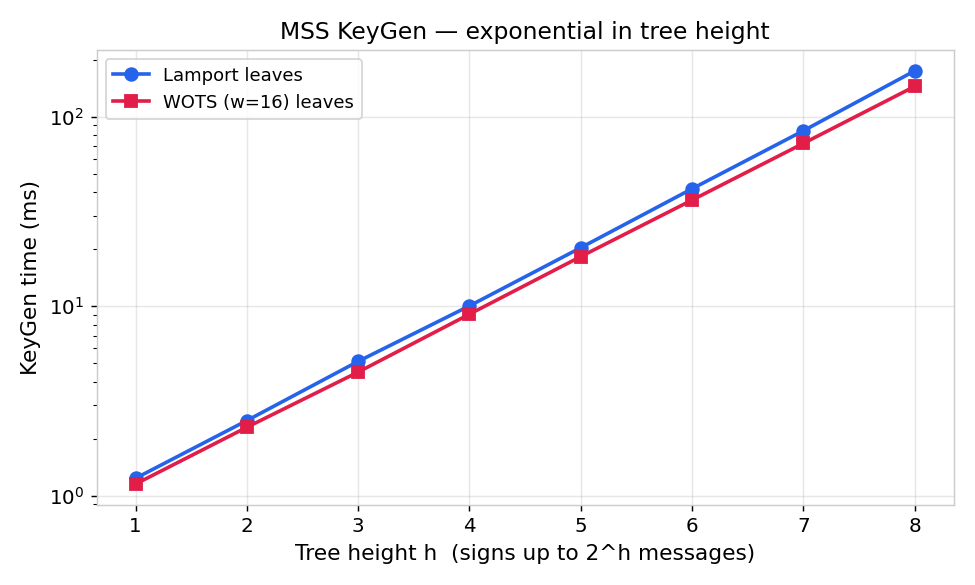
\includegraphics[width=\textwidth]{benchmarks/mss_keygen.png}\\
\footnotesize KeyGen scales as $O(2^h)$: the log-scale plot shows a linear trend.
\end{column}
\begin{column}{0.48\textwidth}
\centering
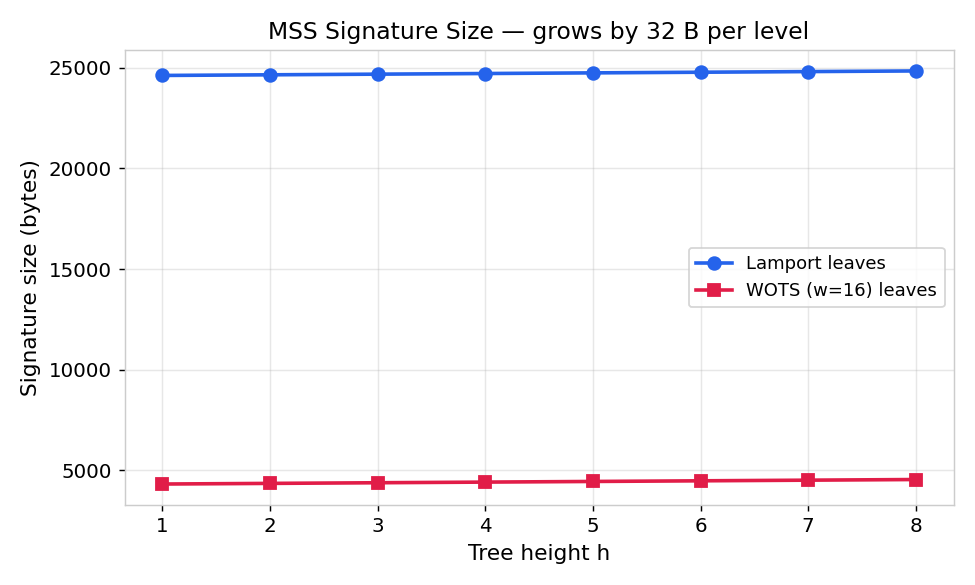
\includegraphics[width=\textwidth]{benchmarks/mss_sig_size.png}\\
\footnotesize Signature size grows by just 32\,B per tree level.
\end{column}
\end{columns}
\end{frame}

% ---- Slide: MSS Sign/Verify ----
\begin{frame}{MSS: Sign \& Verify are Constant-Time in $h$}
\begin{columns}
\begin{column}{0.48\textwidth}
\centering
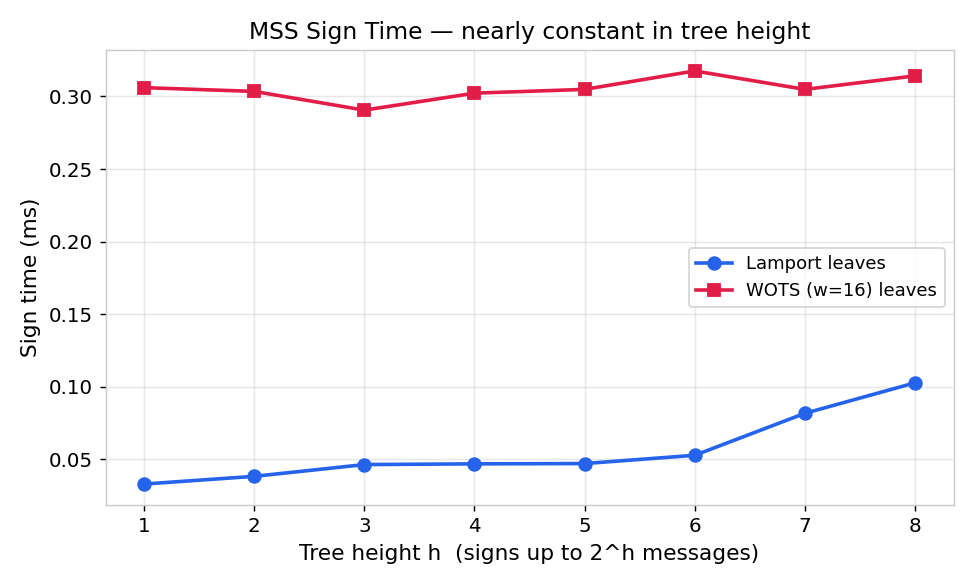
\includegraphics[width=\textwidth]{benchmarks/mss_sign.png}
\end{column}
\begin{column}{0.48\textwidth}
\centering
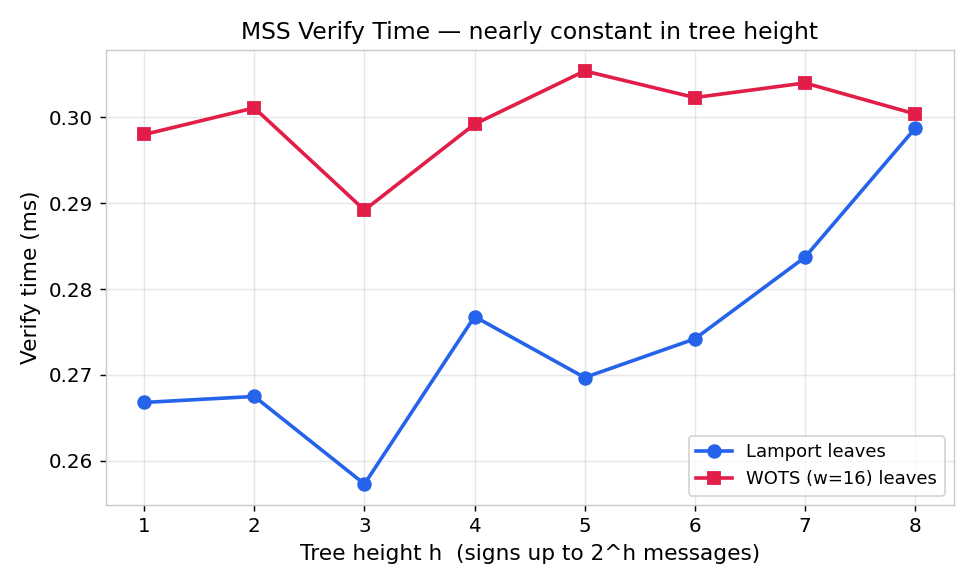
\includegraphics[width=\textwidth]{benchmarks/mss_verify.png}
\end{column}
\end{columns}
\vspace{6pt}
\centering
The $h$ additional hashes for the auth path are negligible compared to the underlying OTS operations.
\end{frame}

% ---- Slide: Parameter Tuning ----
\begin{frame}{Parameter Tuning: MSS with Varying $w$}
\begin{columns}
\begin{column}{0.48\textwidth}
\centering
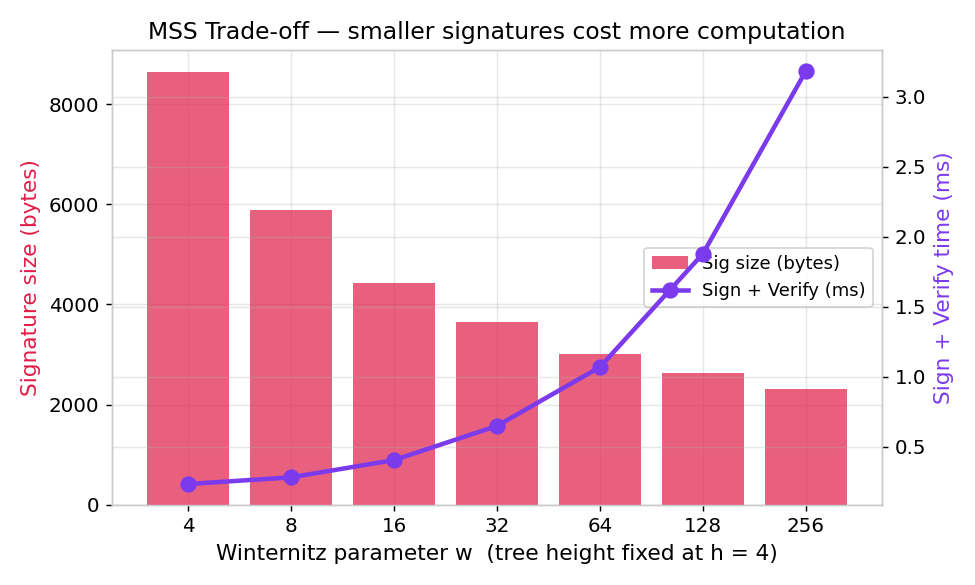
\includegraphics[width=\textwidth]{benchmarks/mss_w_tradeoff.png}
\end{column}
\begin{column}{0.48\textwidth}
\textbf{Fixed:} $h = 4$ (16 messages).\\[6pt]
The \emph{knee} near $w = 16$ marks the optimal balance:
\begin{itemize}
    \item Below $w\!=\!16$: rapid size improvement with modest time cost.
    \item Above $w\!=\!16$: diminishing size returns, escalating time cost.
\end{itemize}

\vspace{8pt}
\begin{block}{Recommendation}
$w = 16$, $h = 4\text{--}8$\\
This matches the XMSS and SPHINCS+ standard configurations.
\end{block}
\end{column}
\end{columns}
\end{frame}

% ---- Slide: Hypertrees (Evaluation section, benchmarks) ----
\begin{frame}{Multi-Layer Merkle Trees (Hypertrees): Performance}
% \textbf{The problem:} Flat MSS KeyGen scales as $O(2^h)$ --- prohibitive at large signing capacities.

% \vspace{4pt}
% \textbf{The idea:} Stack two Merkle trees. The \emph{top} tree's leaves do not sign messages directly; each one certifies the root of a \emph{bottom} tree. Bottom trees are built \alert{lazily}, on demand.
% \begin{itemize}
%     \item Total capacity: $N = 2^{h_{\text{top}} + h_{\text{bot}}}$
%     \item Initial KeyGen: $O(2^{h_{\text{top}}} + 2^{h_{\text{bot}}}) \approx O(\sqrt{N})$
%     \item Same construction used internally by SPHINCS+ / SLH-DSA
% \end{itemize}

\begin{columns}
\begin{column}{0.55\textwidth}
\centering
\scriptsize
\begin{tabular}{lrrr}
\toprule
\textbf{Scheme} & $N$ & \textbf{KG (ms)} & \textbf{Sig (B)} \\
\midrule
Flat MSS, $h\!=\!8$              & 256  & $110.7 \pm 0.6$ & 4{,}548 \\
\rowcolor{success!15}
Hypertree, $h_t\!=\!h_b\!=\!4$    & 256  & $\mathbf{13.8 \pm 0.01}$  & 8{,}876 \\
\midrule
Flat MSS, $h\!=\!10$             & 1024 & $444.9 \pm 4.7$ & 4{,}612 \\
\rowcolor{success!15}
Hypertree, $h_t\!=\!h_b\!=\!5$    & 1024 & $\mathbf{27.4 \pm 0.4}$  & 8{,}940 \\
\bottomrule
\end{tabular}\\[3pt]
\scriptsize Times: mean $\pm$ variance over 5 runs.
\end{column}
\begin{column}{0.42\textwidth}
\centering
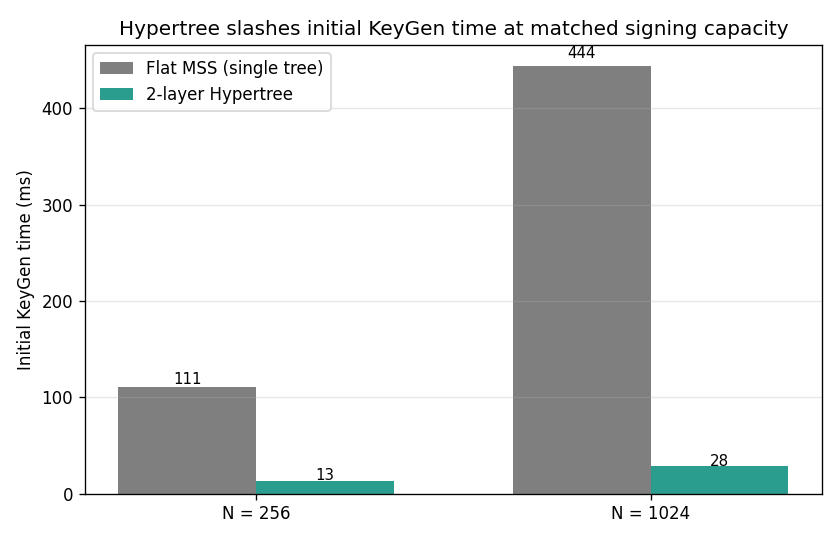
\includegraphics[width=\textwidth]{benchmarks/hypertree_keygen.png}
\end{column}
\end{columns}

\vspace{2pt}
\centering
\footnotesize
\textbf{Result:} 8.0$\times$ faster KeyGen at $N\!=\!256$, 16.2$\times$ faster at $N\!=\!1024$. Signature roughly doubles.
\end{frame}



% ---- Slide: Conclusion ----
\begin{frame}{Conclusion}
\begin{itemize}
    \item We built the full pipeline from scratch using SHA-256: Lamport, WOTS, Merkle Signature Scheme, and a two-layer Hypertree.
    \item WOTS with $w = 16$ is the standard for a reason: four times smaller signatures than Lamport, with manageable speed cost.
    \item Merkle trees lift the one-time restriction: signing and verifying stay constant, and signatures barely grow with tree height.
    \item Hypertrees make the scheme practical at large scale: dramatically faster key generation at the cost of roughly doubling the signature size.
    \item Hash-based signatures rest on only one assumption --- that SHA-256 is one-way --- which is why they remain secure in the post-quantum era.
\end{itemize}
\end{frame}

% ---- Slide: Thank You ----
\begin{frame}{}
\centering
\vspace{2cm}
{\Huge\bfseries Thank You}\\[16pt]
{\Large Questions?}\\[20pt]
\footnotesize
Aicha Slaitane --- \texttt{aicha.slaitane@kaust.edu.sa}\\
Abdullah Algethami --- \texttt{abdullah.algethami@kaust.edu.sa}
\end{frame}

\end{document}
